\documentclass{beamer}

\usepackage[utf8]{inputenc}
\usepackage[portuguese]{babel}
\usepackage{lipsum}
\usepackage{amsmath}
\usepackage{tikz}
\usepackage{multicol}
\usepackage{multirow}
\usepackage[skins]{tcolorbox}
\usepackage{longtable}
\usepackage{booktabs}
\usepackage{ltablex}
\usepackage{listings}


\DeclareUnicodeCharacter{00A0}{~}

\usetheme{Darmstadt} % http://tex.stackexchange.com/questions/177042/beamer-latex-customized-formats
\useoutertheme[subsection=false,footline=authortitle]{miniframes}
% RGB scaled on 0-255 scale (section 17.1.1), colors pulled from title block
\usecolortheme[RGB={8, 80, 135}]{structure}

\title{Processador RISC}
\subtitle{Projeto e implementação em SystemC}
\author[Greati,Vinicius,Artur]{Vitor Greati \inst{1} \and Vinicius Campos\inst{1} \and Artur Curinga\inst{1}}
\institute{
	\inst{1}
	Instituto Metrópole Digital\\
	UFRN
}
\date{Dezembro, 2016}
\subject{Organização e Arquitetura de Computadores}

\AtBeginSection[]
{
  	\begin{frame}
	\frametitle{Conteúdo}
	\tableofcontents[currentsection,currentsubsection]
	\end{frame}
}

\graphicspath{{img/}}

\begin{document}

	\frame{\titlepage}

	\section{Projeto}
		\begin{frame}{Palavra de instrução}

			A programação consiste na listagem de instruções no formato:

			\begin{center}
			\begin{tabular}{|c|c|c|c|}
				\hline
				OPCODE & OD & F1 & F2\\
				4 bits & 9 bits & 9 bits & 9 bits\\
				\hline
			\end{tabular}
			\end{center}
			
			Onde:

			\begin{description}
			    \item [OPCODE] Código da operação
			    \item [OD] Operando Destino (D)
			    \item [F1] Operando Fonte 1 (F1)
			    \item [F2] Operando Fonte 2 (F2)
			\end{description}
		\end{frame}

		\begin{frame}{Conjunto de instruções}

			\begin{table}[H]
			\footnotesize
			\centering
			\begin{tabular}{l | p{6cm} | l}
			Instrução & Ação & Exemplo\\
				\hline
			    LRI & $R[D] \leftarrow F1$ & LRI 1 27\\
			    AND & $D \leftarrow F1 \& F2$ & AND 1 2 3\\
			    OR  & $D \leftarrow F1 | F2$ & OR 1 2 3\\
			    XOR & $D \leftarrow F1 \wedge F2$ & XOR 1 2 3\\
			    NOT & $D \leftarrow \bar{F1}$ & NOT 1 2\\
			    CMP & Z = 1, se $F1==F2$; N = 1, se $F1 < F2$; R[OD] = 0, se $F1 < F2$; R[OD] = 1, se $F1 == F2$, R[OD] = 2, se $F1 > F2$ & CMP 1 2 3\\
			    ADD & $R[D] \leftarrow F1 + F2$ & ADD 1 2 3\\
			    SUB & $R[D] \leftarrow F1 - F2$ & SUB 1 2 3\\
			    LD  & $R[D] \leftarrow MEM[F1]$ & LD 1 2\\
			    ST  & $MEM[D] \leftarrow R[F1]$ & ST 1 2\\
			    J   & $CP \leftarrow F1$ & J 23\\
			    JN  & $CP \leftarrow F1 \text{ if } N == 1$ & JN 23\\
			    JZ  & $CP \leftarrow F1 \text{ if } Z == 1$ & JZ 23\\
			\end{tabular}
			\label{tab:inst}
			\caption{Conjunto de instruções.}
			\end{table}
		\end{frame}

		\begin{frame}{Modos de endereçamento}

			Permitem-se três modos de endereçamento:

			\begin{block}{Direto}
			    É fornecido o endereço da memória de dados
			    que se deseja manipular. Apenas instruções \textbf{LD} e \textbf{ST} podem referenciar diretamente a memória.
			\end{block}

			\begin{block}{Registrador direto}
			    É fornecido o endereço do
			    registrador com que se deseja trabalhar.
			\end{block}

			\begin{block}{Registrador imediato}
			    É fornecido o endereço
			    do registrador e um valor imediato a ser inserido
			    nele.
			\end{block}

		\end{frame}
		
		\begin{frame}{Memórias}
			
			\begin{block}{Registradores}
			Há 32 registradores disponíveis para palavras de 32 bits.
			\end{block}

			\begin{block}{Memória de instruções}
			256 palavras de 32 bits.
			\end{block}

			\begin{block}{Memória de dados}
			512 palavras de 32 bits.
			\end{block}

		\end{frame}

		\begin{frame}{Barramentos}
			\begin{block}{Controle}
			Transmite os sinais de controle para
			a parte operativa.
			\end{block}

			\begin{block}{Dados}
			Transmite as palavras de dados de 32 bits.
			\end{block}

			\begin{block}{Endereços}
			Transmite os endereços utilizados nas
			leituras e escritas em memória, com largura de 8 bits.
			\end{block}
		\end{frame}

		\begin{frame}{Pipeline}
			\begin{itemize}
				\item<1-> Apenas dois estágios: entre a busca e a execução;
				\item<2-> Um registrador guarda a palavra de instrução decodificada;
				\item<3-> É pessimista: sempre que ocorre uma intrução de \emph{jump},
					desconsidera a instrução pré-carregada;
				\item<4-> Ainda que simples, demonstrou redução visível nos ciclos, como
					mostrado nos testes mais adiante.
			\end{itemize}
		\end{frame}


	\section{Diagramas}
	
		\begin{frame}{Parte operativa}
			\begin{figure}[H]
				\centering
				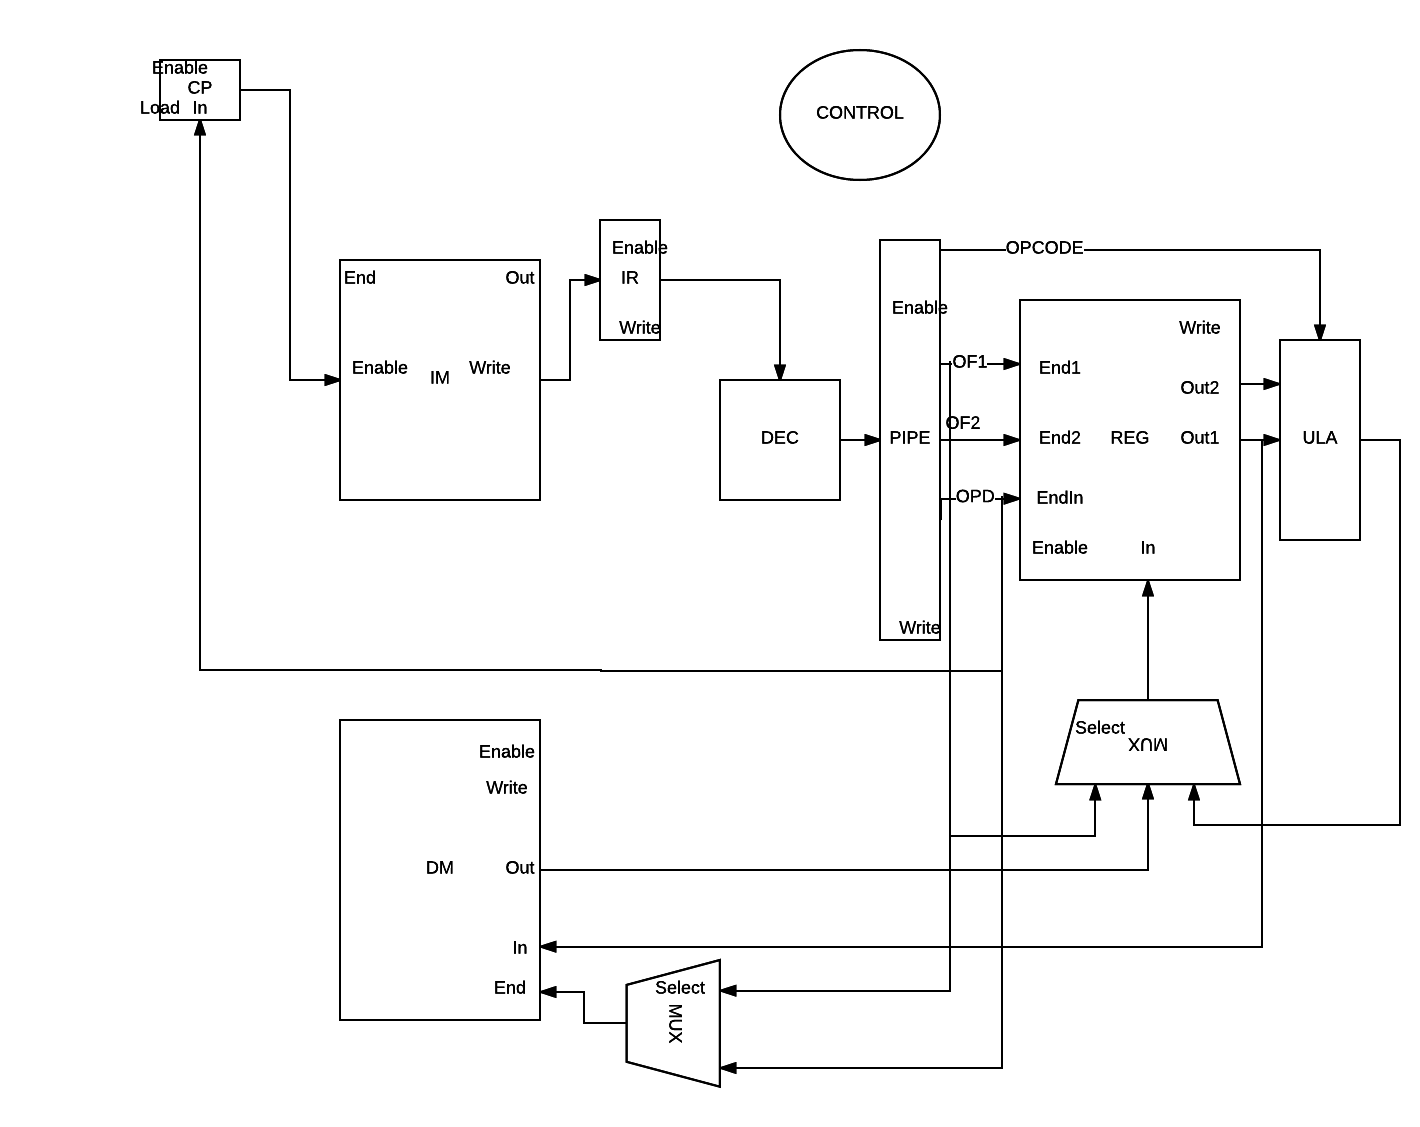
\includegraphics[scale=0.4]{img/procdiag}
			\end{figure}
		\end{frame}

		\begin{frame}{Parte de controle}

			{\footnotesize
				A parte de controle consiste em um bloco que recebe a palavra de instrução decodificada
			e utiliza uma máquina de estados para gerar os sinais de controle adequados
			a cada microinstrução. 
			}
			\begin{figure}[H]
				\centering
				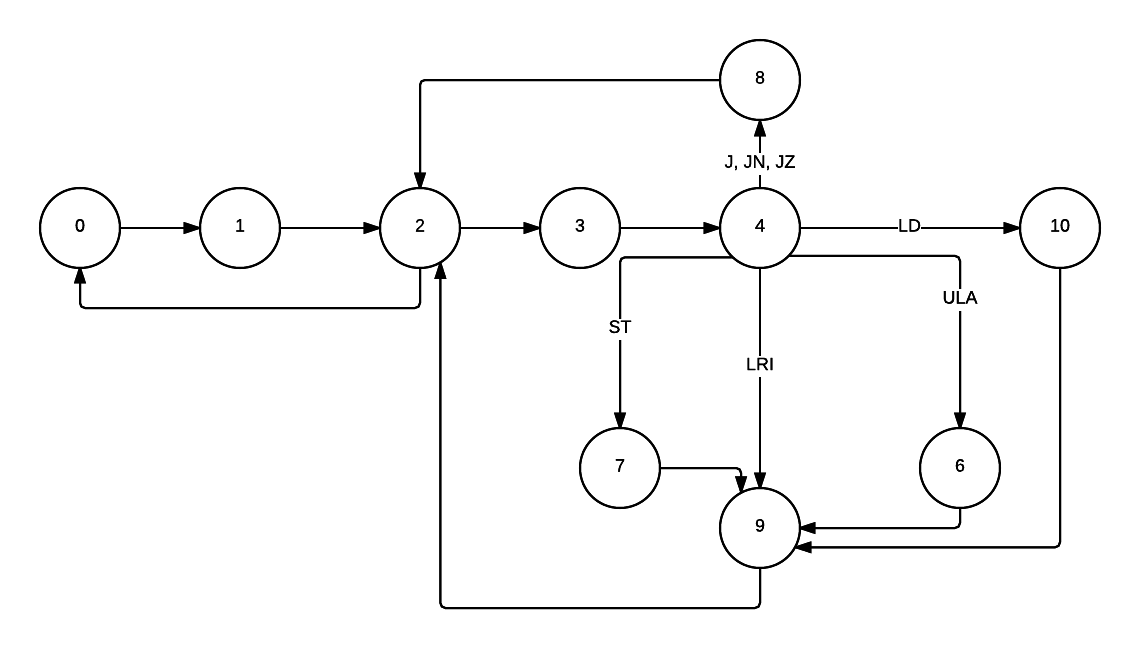
\includegraphics[scale=0.5]{img/statediag}
			\end{figure}

		\end{frame}

		\begin{frame}{Estados}
			A tabela abaixo descreve o que ocorre em cada estado:

			\begin{table}[H]
				\footnotesize
				\centering
				\begin{tabular}{l | p{7cm}}
					Estado	& Ações\\
					\hline
					0	& Prepara para escrever a instrução no barramento.\\
					1	& Prepara para escrever a instrução no RI.\\
					2	& Caso o pipeline não seja reiniciado, prepara para escrever no
						  registrador de pipeline. Caso seja, envia para o estado 0.\\
					3	& Desabilita escrita no pipeline, prepara nova instrução para o
						  barramento do RI (pipelining).\\
					4 	& Prepara a execução da instrução de fato e a escrita no RI da 
						  próxima instrução (pipelining).\\
					6	& Desabilita sinais após a execucação da ULA.\\
					7	& Desabilita sinais após a escrita na memória.\\
					8	& Desabilita escrita no CP e envia para o estado 2, para
						  reiniciar o processo.\\
					9	& Desabilita sinais após guardar os resultados no banco de registradores.\\
					10	& Prepara execução da operação de LD.\\
					\hline
				\end{tabular}
			\end{table}
		\end{frame}

	\section{Implementação}
		
	\begin{frame}{Implementação}
		\begin{itemize}
			\item<1-> Biblioteca SystemC 2.3.1;
			\item<2-> Cada módulo implementado separadamente, mantendo boa organização;
			\item<3-> O programa recebe um arquivo com um algoritmo escrito segundo as
				instruções da arquitetura;
			\item<4-> Para executar:
				{\ttfamily ./processador\_run instrucoes.txt}
		\end{itemize}
	\end{frame}

	\section{Testes}
	\begin{frame}{Execuções individuais}
		Primeiro, testamos cada instrução separadamente, obtendo o número de ciclos
		que cada uma toma, \textbf{considerando a identificação de parada}:

		\begin{table}[H]
		\footnotesize
		\centering
		\begin{tabular}{l | r}
		Instrução & Ciclos\\
			\hline
		    AND & 9\\ 
		    OR  & 9\\
		    XOR & 9\\
		    NOT & 9\\
		    CMP & 9\\
		    ADD & 9\\
		    SUB & 9\\
		    LD  & 9\\
		    ST  & 9\\
		    J   & 11\\
		    JN  & 11\\
		    JZ  & 11\\
		    LRI & 9\\
		\end{tabular}
		\label{tab:insttest}
		\caption{Ciclos para cada instrução.}
		\end{table}
	\end{frame}

	\begin{frame}{Algoritmos para testes}
		Para testar o funcionamento do processador e do pipeline, os seguintes algoritmos foram utilizados:\\
		\begin{block}{3x6}
		{\footnotesize
		LRI 1 3\\
		LRI 2 6\\
		LRI 3 1\\
		LRI 4 0\\
		LRI 5 0\\
		CMP 9 4 1\\
		JZ 10\\
		ADD 5 5 2\\
		SUB 1 1 3\\
		J 5\\
		ST 1 5\\
		}
		\end{block}
	\end{frame}

	\begin{frame}{Algoritmos para testes}

		Computa o décimo elemento da sequência de Fibonacci e o armazena na memória:\\
		\begin{block}{Fib(10)}
		{\scriptsize
		LRI 3 1\\    
		LRI 6 0\\ 
		LRI 7 1\\   
		LRI 1 0\\   
		LRI 2 1\\  
		LRI 4 1\\   
		LRI 5 10\\  
		SUB 5 5 7\\ 
		CMP 9 5 4\\ 
		JN 15\\	  
		ADD 3 1 2\\ 
		ADD 1 6 2\\ 
		ADD 2 6 3\\ 
		ADD 4 7 4\\ 
		J 8\\	
		ST 1 3\\
		}
		\end{block}
	\end{frame}

	\begin{frame}{Algoritmos para testes}
			Realiza todas as operações lógicas possíveis com o processador
				em operandos advindos da memória de dados:\\
		\begin{block}{Logic}
		{\footnotesize
		LRI 0 2\\
		LRI 1 3\\
		ST 0 0\\
		ST 1 1\\
		LD 2 0\\
		LD 3 1\\
		ADD 4 3 2\\
		SUB 5 4 3\\
		AND 6 1 2\\
		OR 7 1 2\\
		XOR 8 1 2\\
		NOT 9 1\\
		}
		\end{block}

	\end{frame}

	\begin{frame}{Resultados dos algoritmos}
		\begin{table}[H]
			\centering
			\begin{tabular}{c | c | c}

			Algoritmo	& Ciclos sem pipeline	& Ciclos com pipeline\\
			\hline
			3x6		& 149			& 115		     \\
			Fib(10)		& 492			& 374		     \\
			Logic	        & 82			& 58		     \\
			\hline
			\end{tabular}
			\caption{Resultados de execução dos algoritmos de teste.}
			\label{tab:resultados}
		\end{table}
	\end{frame}

	\section{Conclusões}
	\begin{frame}{Conclusões}
		\begin{itemize}
			\item<1-> Implementou-se um processador simples, mas
			funcional, unindo conceitos da disciplina de OAC e de Circuitos
			Lógicos;
		\item<2-> Ainda com um \emph{pipeline} simplificado, foi visível a 
			redução no ciclo de instruções, validando o poder dessa técnica;
		\item<3-> O projeto consolidou os conceitos
			aprendidos nas aulas teóricas, além de mostrar
			como se pode descrever \emph{hardware} de forma
			ainda mais abstrata.
		\end{itemize}
	\end{frame}

\end{document}
